\documentclass{article}
\input{../../../../../../LaTex/preamble/preamble_article.tex}


\title{专项训练}
\author{学生: 王一帆 \quad 教师: 马祥芸}


\begin{document}
\maketitle
\tableofcontents
\zihao{-4}
\newpage

\section{运动图像问题}
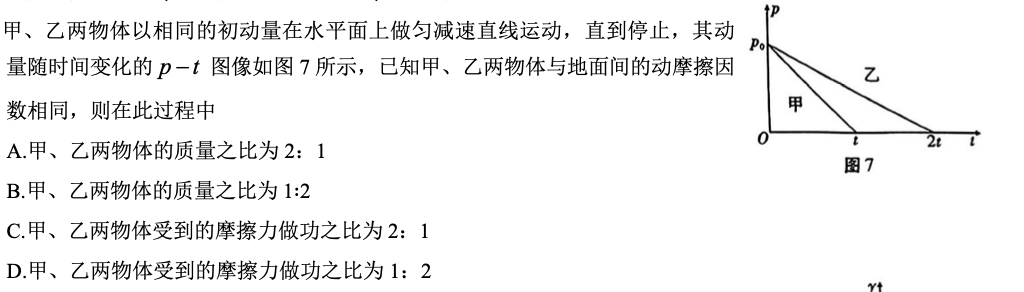
\includegraphics[width = 0.95\textwidth]{./pictures/1.png}

\vspace{5em}

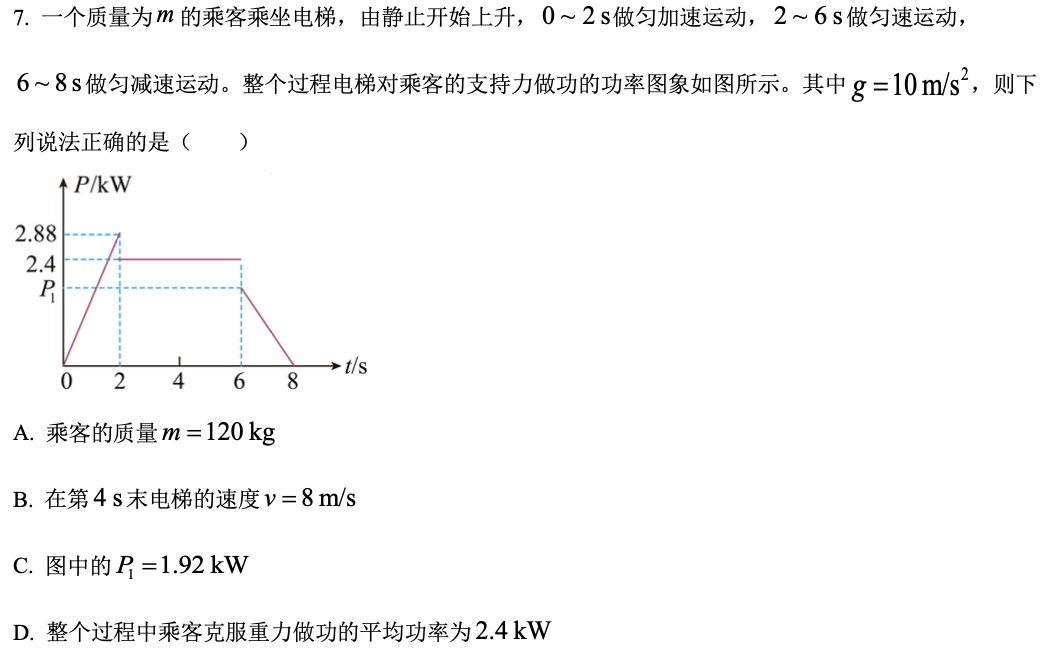
\includegraphics[width = 0.95\textwidth]{./pictures/2.png}

\vspace{5em}

\section{原子核物理}
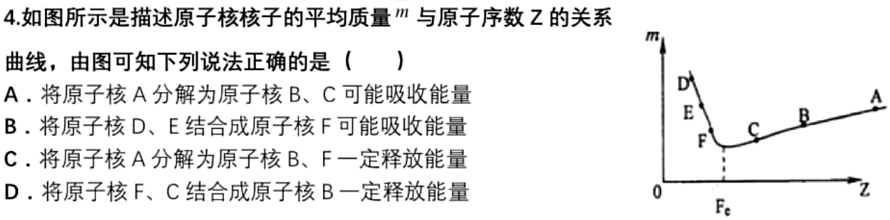
\includegraphics[width = 0.95\textwidth]{./pictures/3.png}

\vspace{5em}

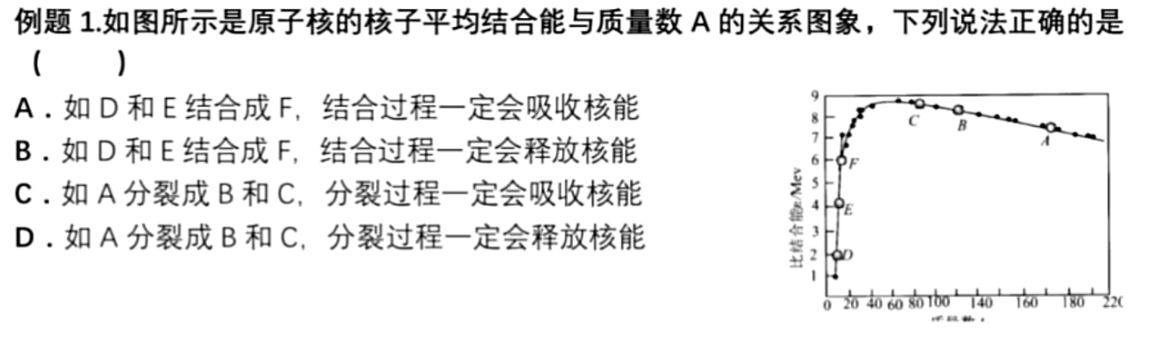
\includegraphics[width = 0.95\textwidth]{./pictures/4.png}

\vspace{5em}

\section{万有引力}
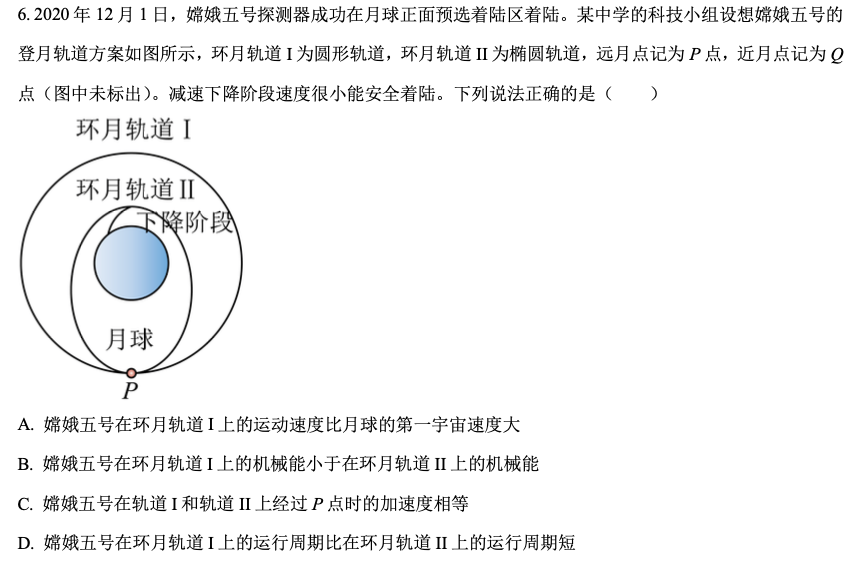
\includegraphics[width = 0.95\textwidth]{./pictures/5.png}

\vspace{5em}

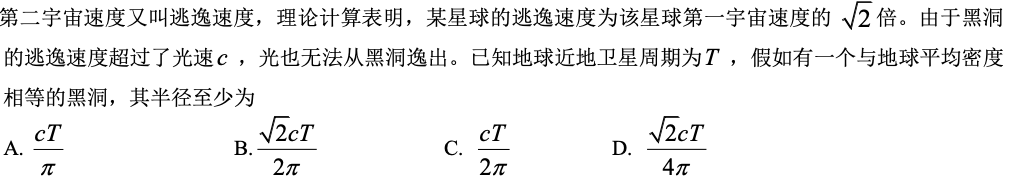
\includegraphics[width = 0.95\textwidth]{./pictures/6.png}

\vspace{5em}

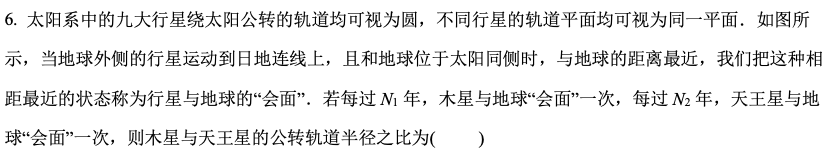
\includegraphics[width = 0.95\textwidth]{./pictures/7-1.png}

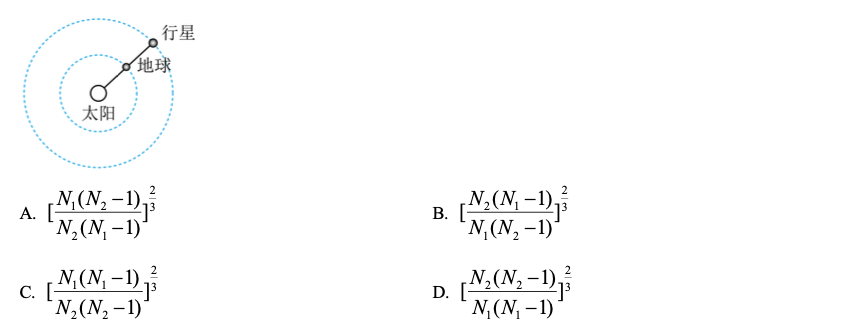
\includegraphics[width = 0.95\textwidth]{./pictures/7-2.png}

\vspace{5em}

\section{霍尔元件}
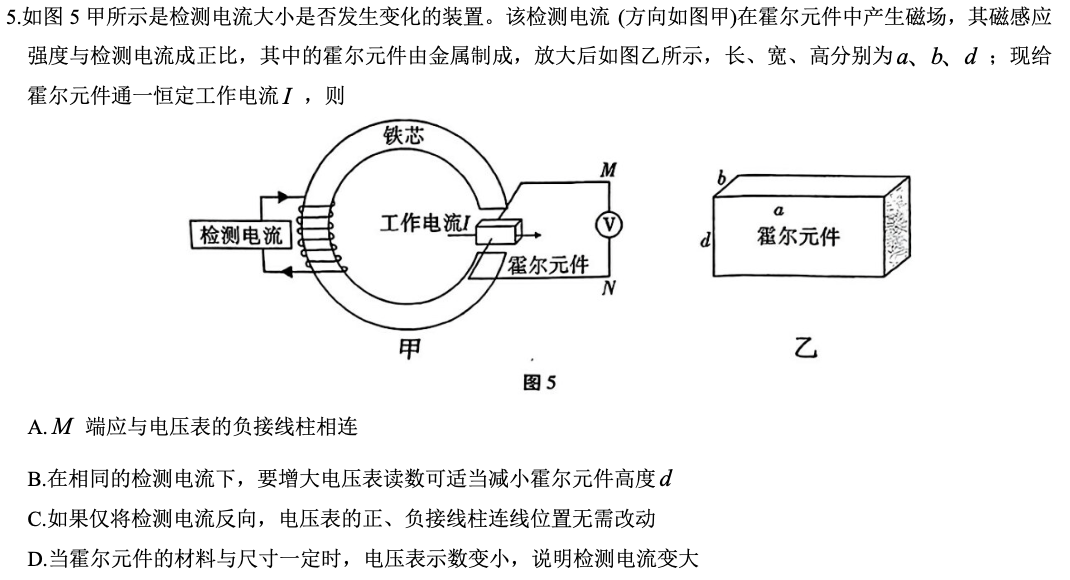
\includegraphics[width = 0.95\textwidth]{./pictures/8.png}

\vspace{5em}

\begin{minipage}{0.45\textwidth}
    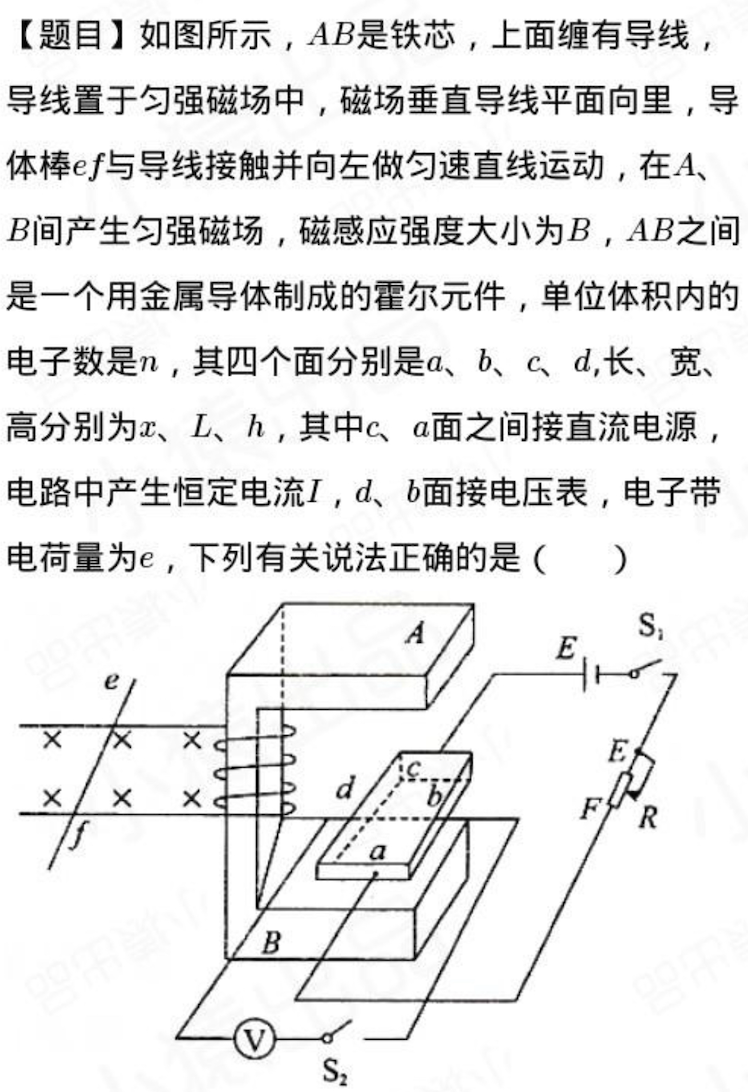
\includegraphics[width=\textwidth,keepaspectratio]{./pictures/9-1.png}
\end{minipage}
\hfill
\begin{minipage}{0.45\textwidth}
    \vspace{-20em}
    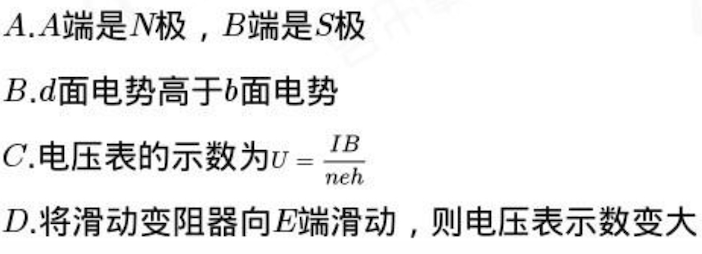
\includegraphics[width=\textwidth,keepaspectratio]{./pictures/9-2.png}
\end{minipage}

\vspace{5em}

\section{动态受力分析}
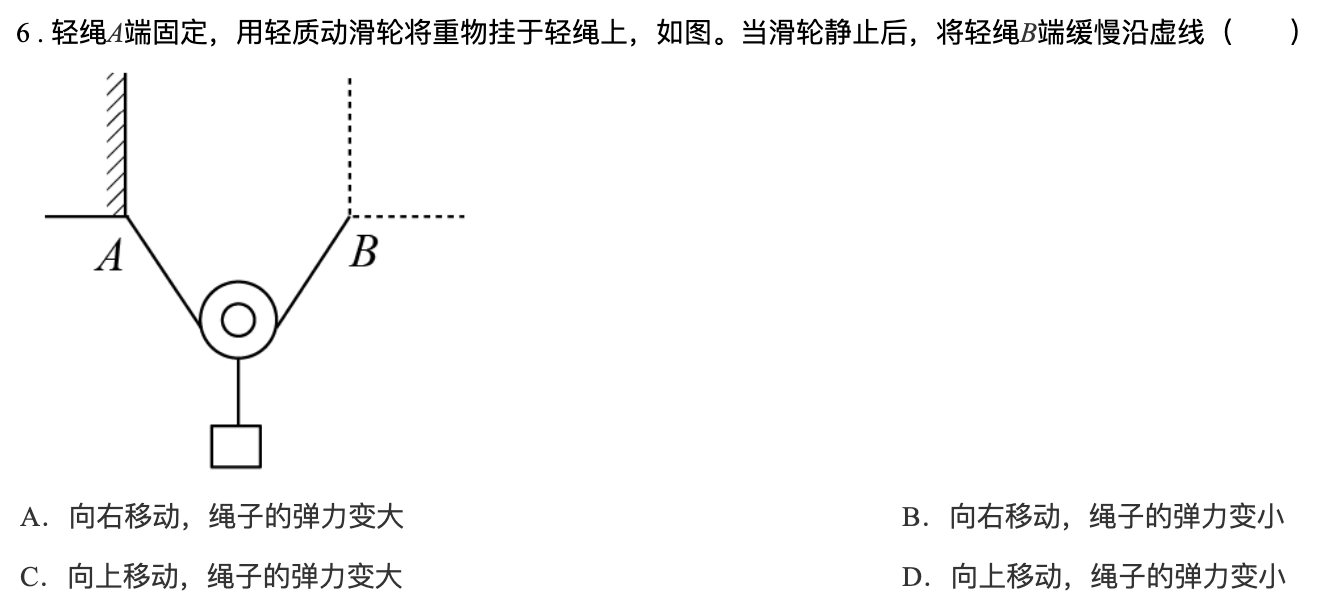
\includegraphics[width = 0.95\textwidth]{./pictures/10.png}

\vspace{5em}

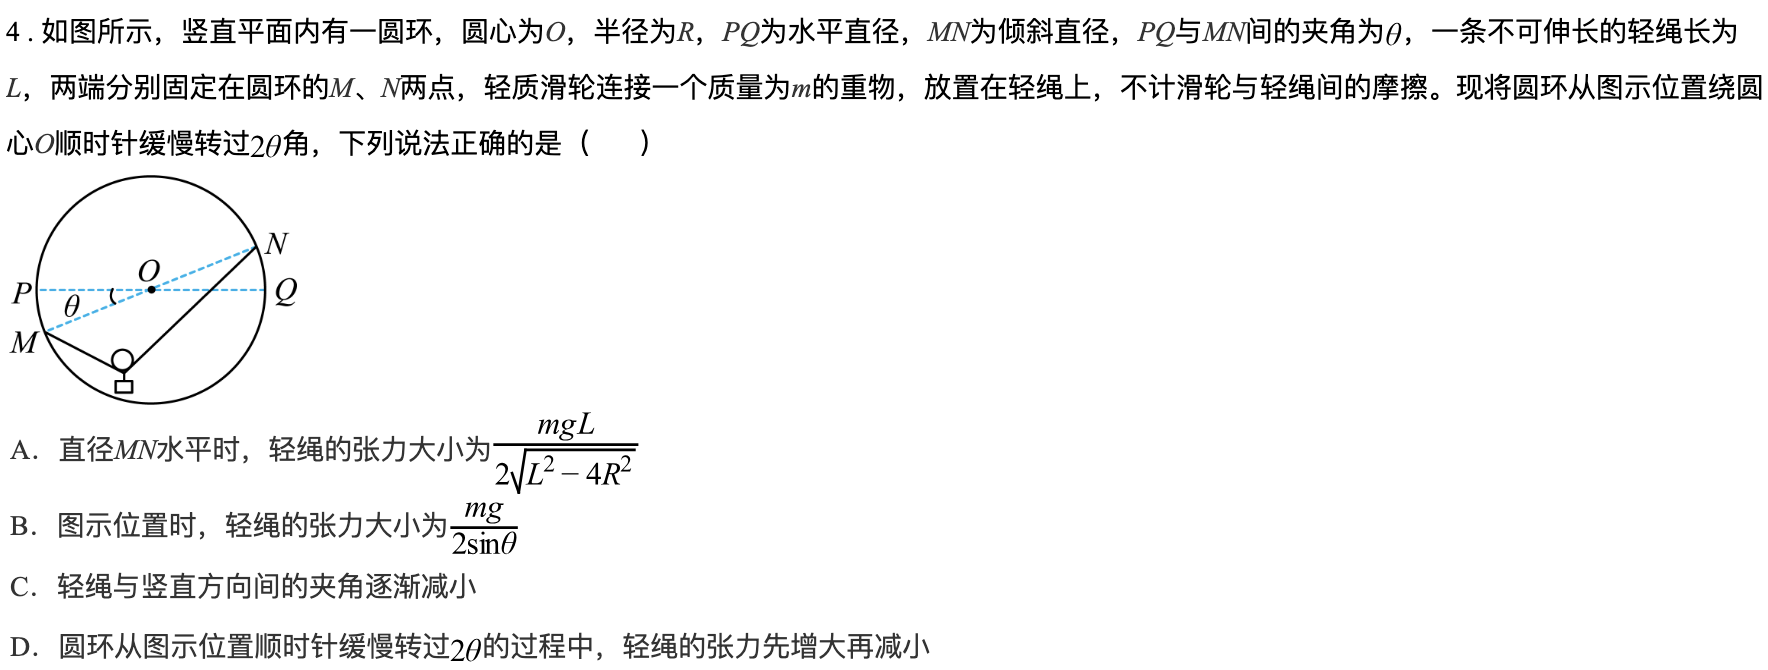
\includegraphics[width = 0.95\textwidth]{./pictures/11.png}

\vspace{5em}

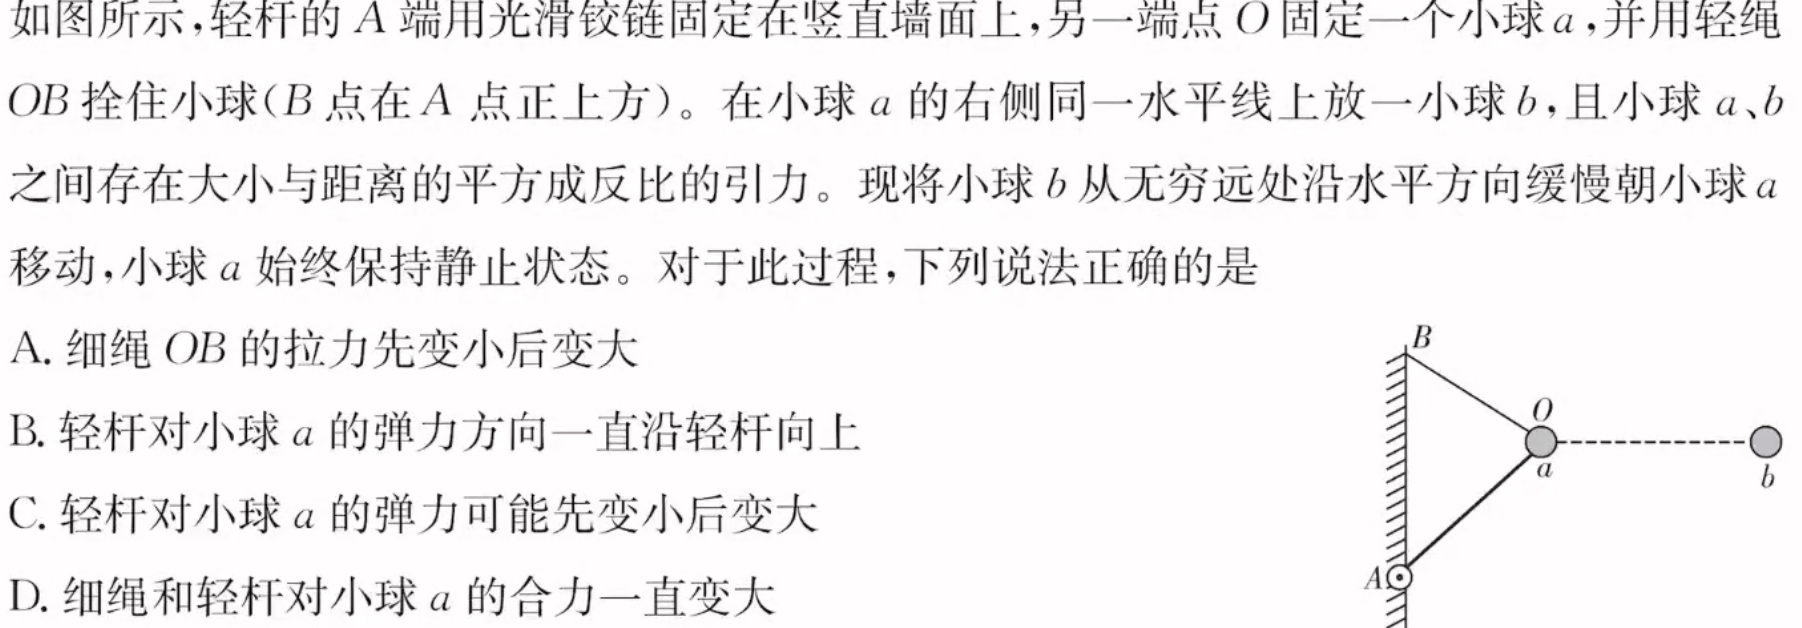
\includegraphics[width = 0.95\textwidth]{./pictures/12.png}

\vspace{5em}

\section{绳的关联速度}
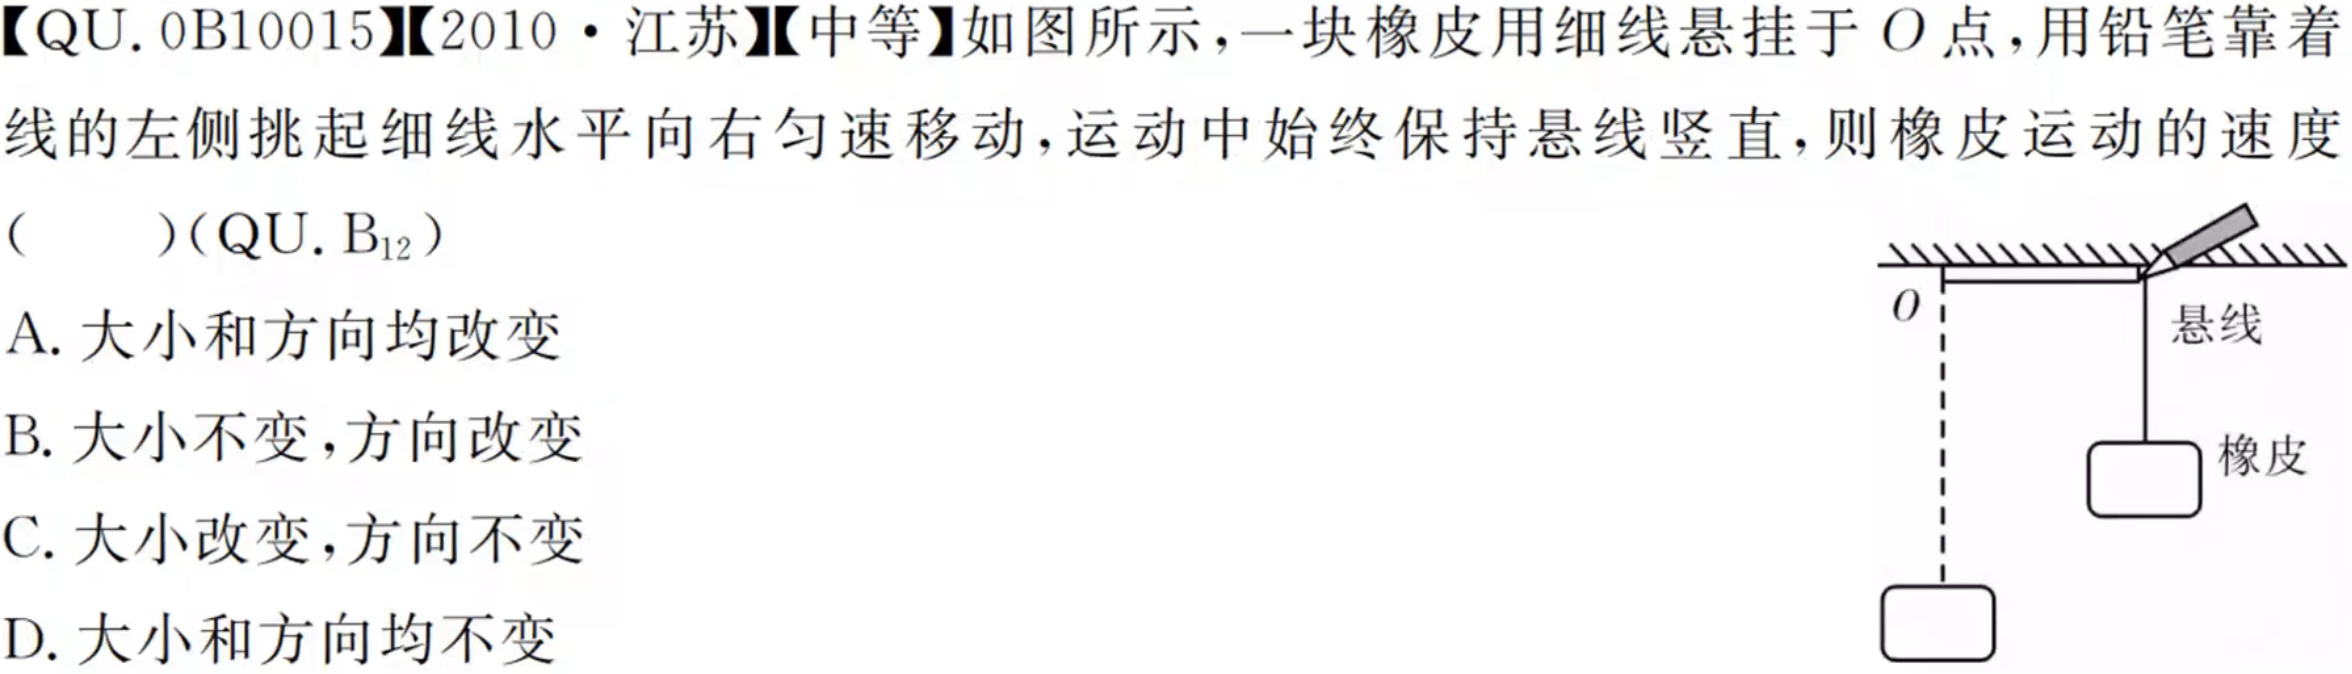
\includegraphics[width = 0.95\textwidth]{./pictures/13.png}

\vspace{5em}

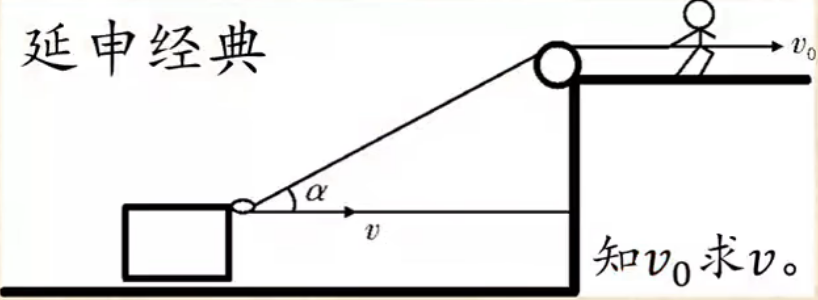
\includegraphics[width = 0.8\textwidth]{./pictures/14.png}

\vspace{5em}

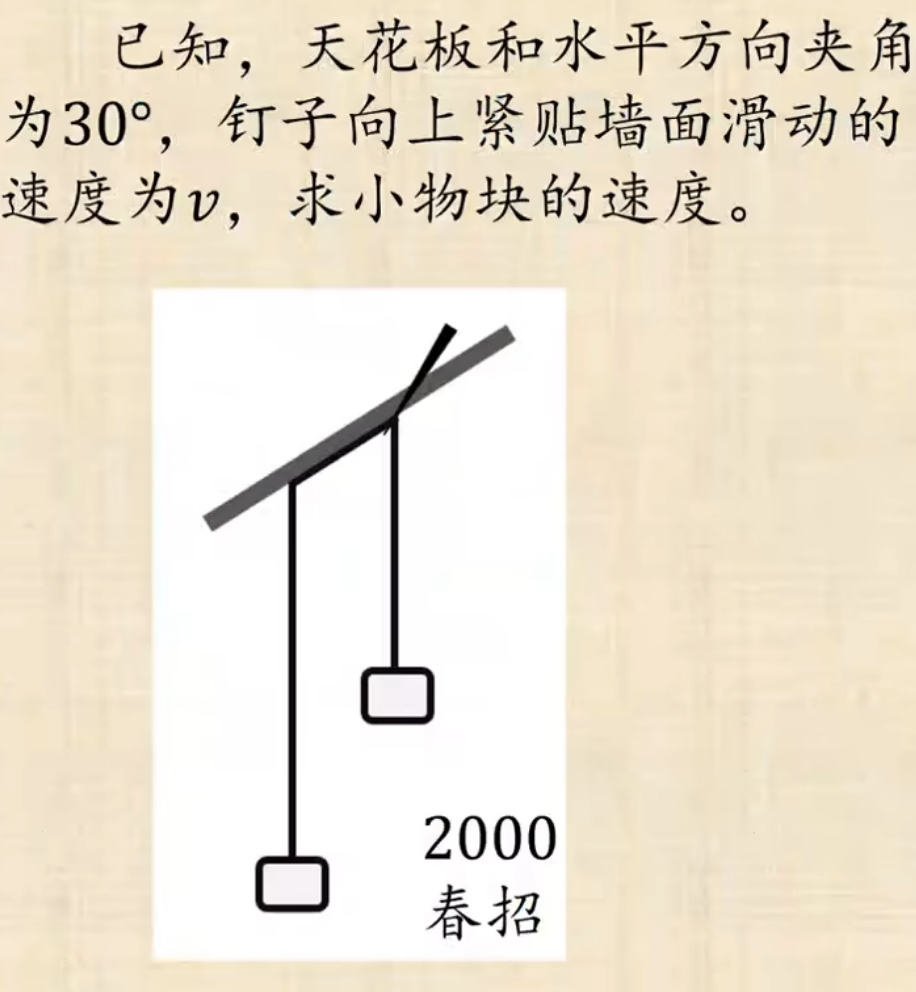
\includegraphics[width = 0.8\textwidth]{./pictures/15.png}

\vspace{5em}

\section{机械波与简谐运动}
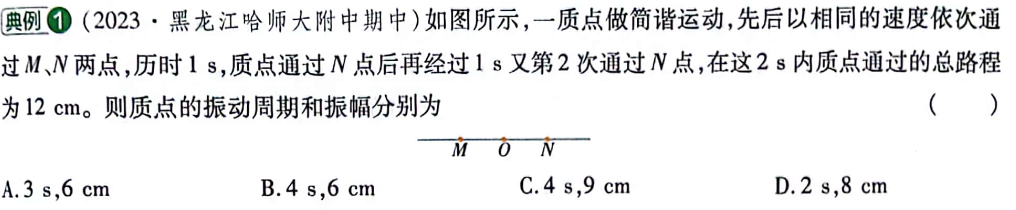
\includegraphics[width = 0.8\textwidth]{./pictures/16.png}

\vspace{5em}

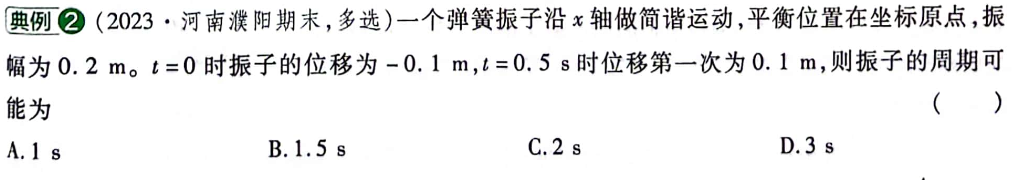
\includegraphics[width = 0.8\textwidth]{./pictures/17.png}

\vspace{5em}

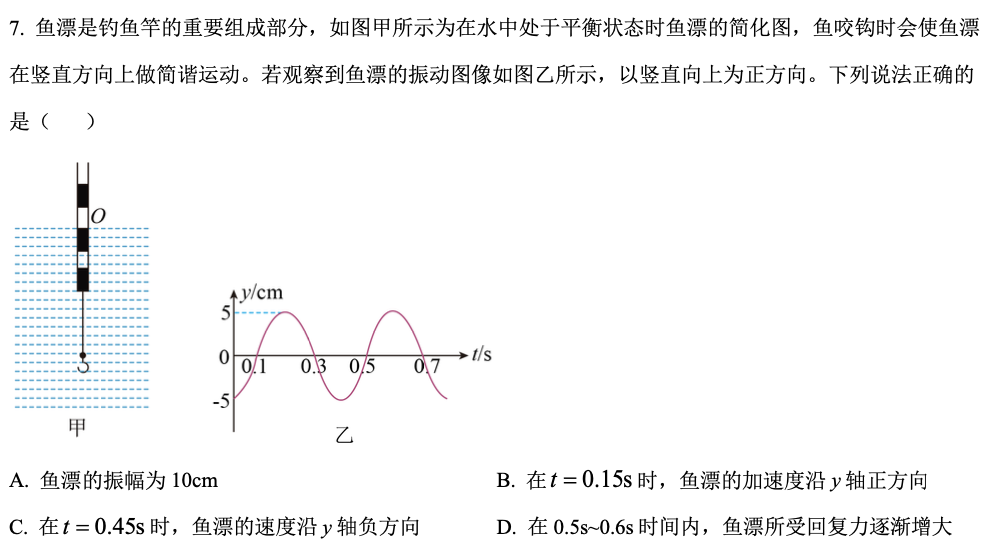
\includegraphics[width = 0.8\textwidth]{./pictures/18.png}

\vspace{5em}

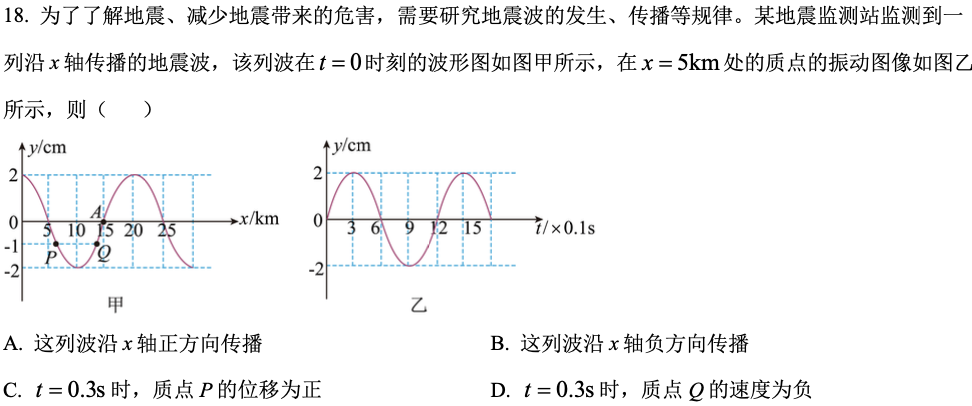
\includegraphics[width = 0.8\textwidth]{./pictures/19.png}

\vspace{5em}

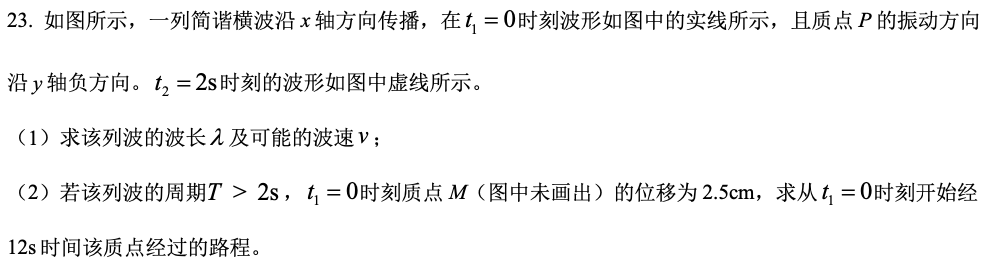
\includegraphics[width = 0.8\textwidth]{./pictures/20.png}

\vspace{5em}

\section{折射率}
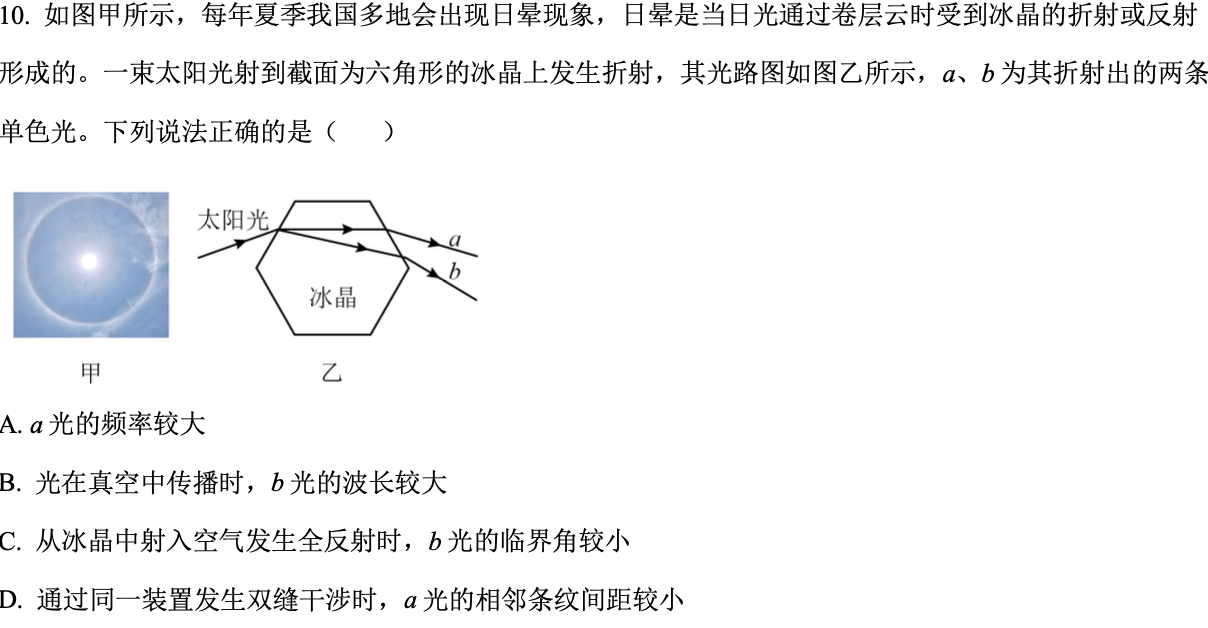
\includegraphics[width = 0.9\textwidth]{./pictures/24.png}

\vspace{5em}

符号说明

\begin{tabular}{|c|c|c|c|c|c|c|c|c|c|}
    \hline
    频率  & 折射率 & 速度  & 临界角 & 波长        & 动量  & 干涉            & 能量            & 逸出功     & 逃逸光子动能  \\
    \hline
    $f$ & $n$ & $v$ & $C$ & $\lambda$ & $p$ & $\triangle x$ & $\varepsilon$ & $w_{0}$ & $E_{k}$ \\
    \hline
\end{tabular}

\vspace*{2em}

\begin{itemize}
    \item 同一介质中不同频率的光

          \vspace*{1em}
          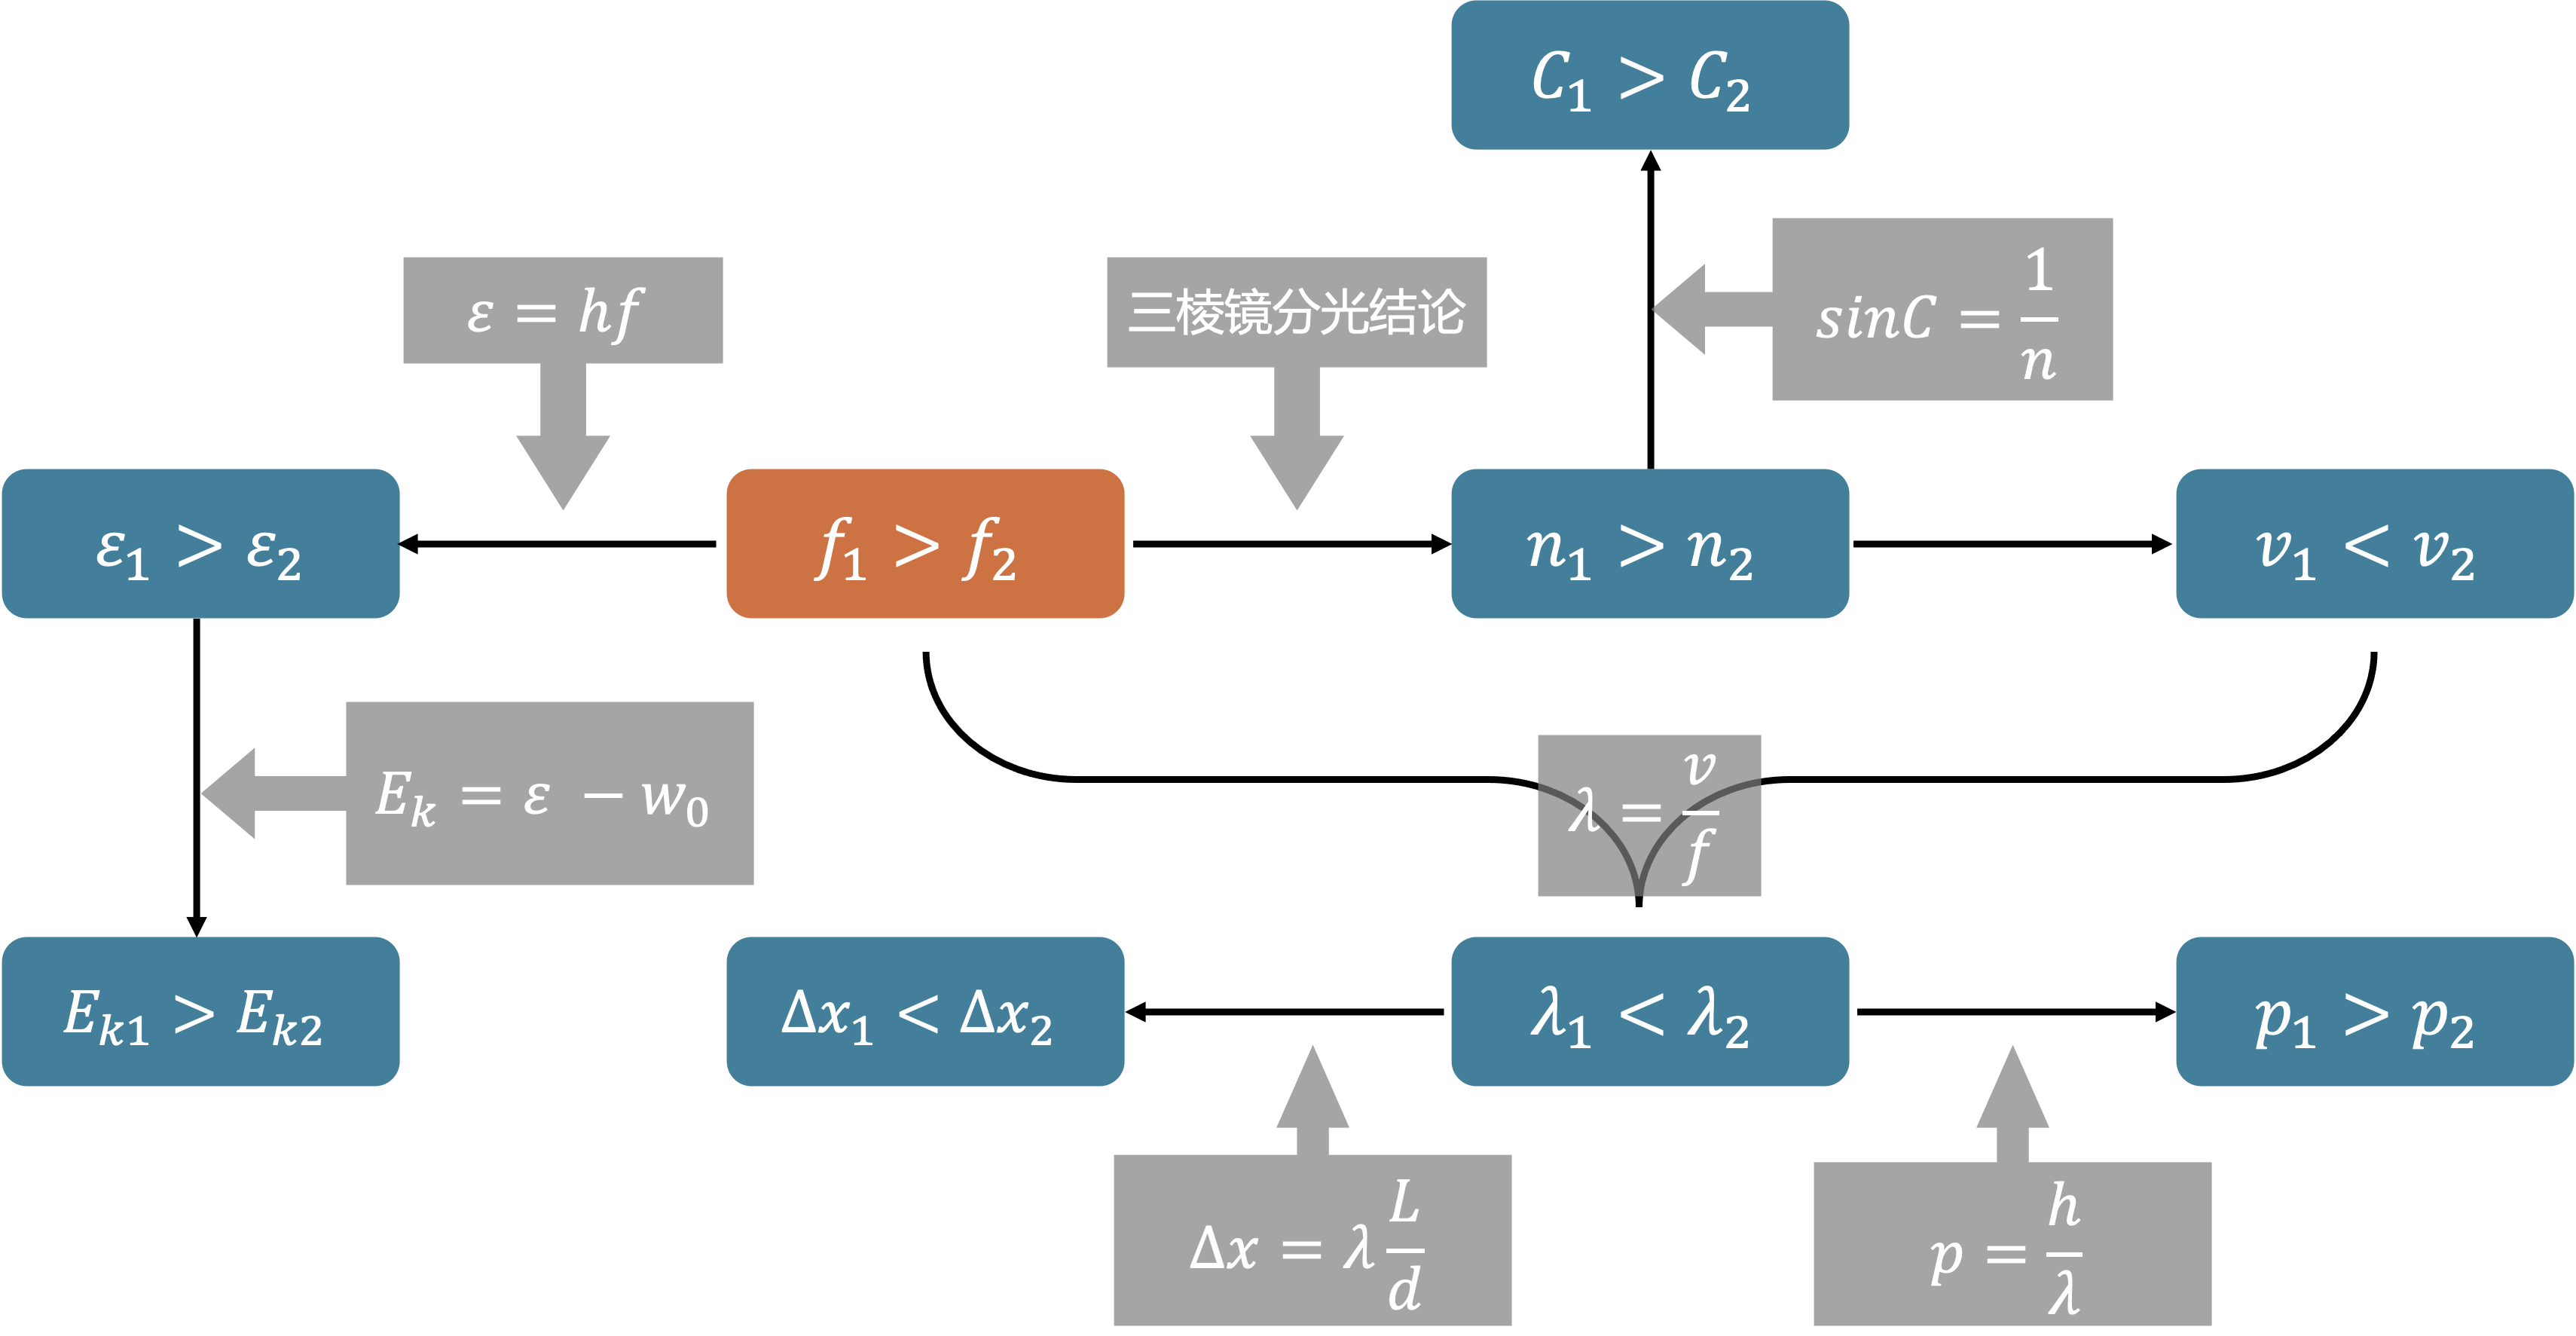
\includegraphics[width=35em,keepaspectratio]{./pictures/22.png}

          \vspace*{2em}

    \item 同一频率的光在不同介质(下标表示不同介质中)中

          \vspace*{1em}
          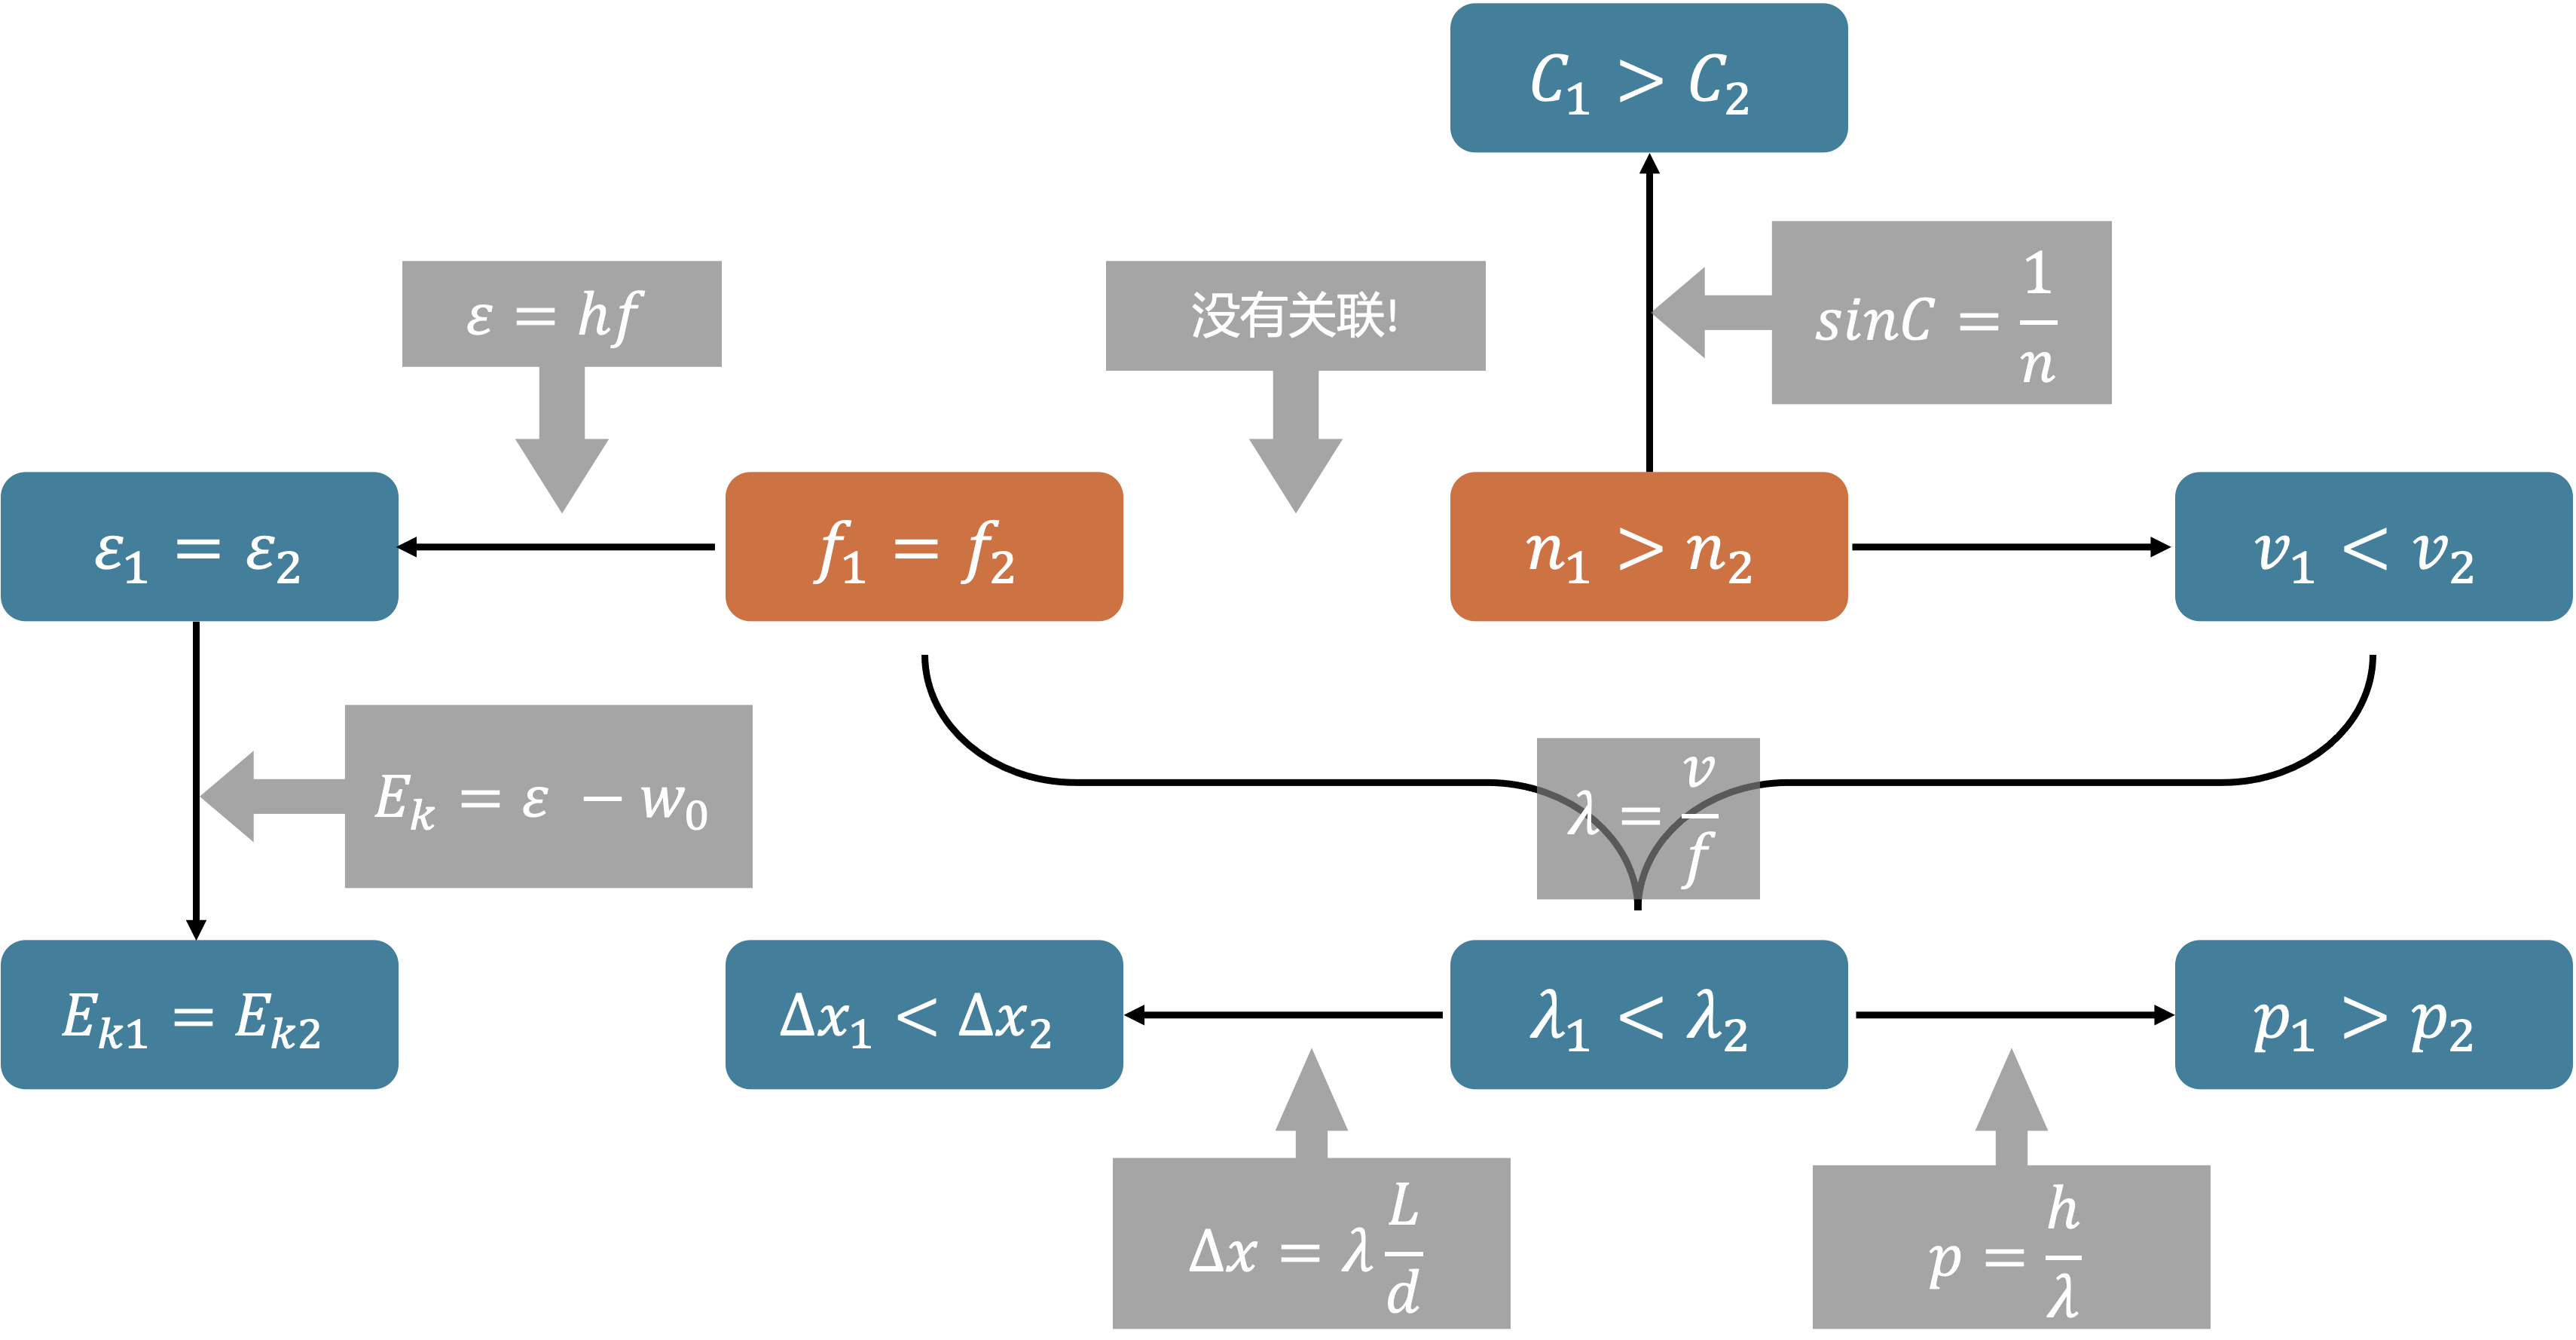
\includegraphics[width=35em,keepaspectratio]{./pictures/23.png}
\end{itemize}

\vspace{5em}

\section{非重力场问题}
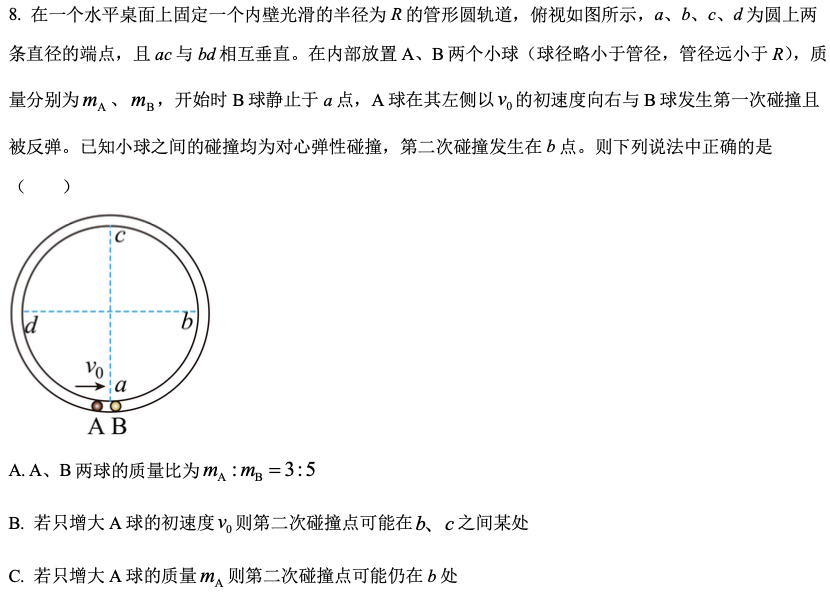
\includegraphics[width = 0.9\textwidth]{./pictures/21-1.png}

\hspace{0.2em}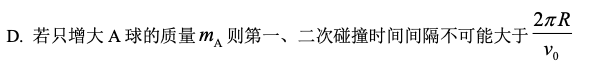
\includegraphics[width = 0.6\textwidth]{./pictures/21-2.png}




\newpage

\section{参考答案}

\begin{minipage}{0.5\textwidth}
    \begin{itemize}
        \item 运动图像问题
              \begin{enumerate}
                  \item AD
                  \item C
              \end{enumerate}
        \item 原子核物理
              \begin{enumerate}
                  \item C
                  \item BD
              \end{enumerate}
        \item 万有引力
              \begin{enumerate}
                  \item C
                  \item D
                  \item A
              \end{enumerate}
        \item 霍尔元件
              \begin{enumerate}
                  \item B
                  \item ABC
              \end{enumerate}
        \item 动态受力分析
              \begin{enumerate}
                  \item A
                  \item AD
                  \item CD
              \end{enumerate}
        \item 绳的关联速度
              \begin{enumerate}
                  \item D
                  \item $v = \frac{v_{0}}{1+\cos{\alpha}}$
                  \item $\sqrt{3}v$
              \end{enumerate}
        \item 机械波与简谐运动
              \begin{enumerate}
                  \item B
                  \item AD
                  \item D
                  \item AC
                  \item \begin{itemize}
                    \item[(1)] $8m$ 
                    \item[(2)] $(4n+1) \, m/s$
                    \item[(3)] $30 \, cm$
                  \end{itemize}
              \end{enumerate}
        \item 折射率
              \begin{enumerate}
                  \item C
              \end{enumerate}
        \item 非重力场
              \begin{enumerate}
                  \item CD
              \end{enumerate}
    \end{itemize}
\end{minipage}















\end{document}